\documentclass{article}

%\usepackage{fullpage}

%-------------------------------------------------------------------------------
%          -Packages nécessaires pour écrire en Français et en UTF8-
%-------------------------------------------------------------------------------
\usepackage[utf8]{inputenc}
\usepackage[frenchb]{babel}
\usepackage[T1]{fontenc}
\usepackage{lmodern}
\usepackage{textcomp}



%-------------------------------------------------------------------------------

%-------------------------------------------------------------------------------
%                          -Outils de mise en forme-
%-------------------------------------------------------------------------------
\usepackage{hyperref}
\hypersetup{pdfstartview=XYZ}
%\usepackage{enumerate}
\usepackage{graphicx}
\usepackage{multicol}
\usepackage{tabularx}
\usepackage{multirow}


\usepackage{anysize} %%pour pouvoir mettre les marges qu'on veut
%\marginsize{2.5cm}{2.5cm}{2.5cm}{2.5cm}

\usepackage{indentfirst} %%pour que les premier paragraphes soient aussi indentés
\usepackage{verbatim}
\usepackage{enumitem}
\usepackage[usenames,dvipsnames,svgnames,table]{xcolor}

\usepackage{variations}

%-------------------------------------------------------------------------------


%-------------------------------------------------------------------------------
%                  -Nécessaires pour écrire des mathématiques-
%-------------------------------------------------------------------------------
\usepackage{amsfonts}
\usepackage{amssymb}
\usepackage{amsmath}
\usepackage{amsthm}
\usepackage{tikz}
\usepackage{xlop}
%-------------------------------------------------------------------------------



%-------------------------------------------------------------------------------


%-------------------------------------------------------------------------------
%                    - Mise en forme avancée
%-------------------------------------------------------------------------------

\usepackage{ifthen}
\usepackage{ifmtarg}


\newcommand{\ifTrue}[2]{\ifthenelse{\equal{#1}{true}}{#2}{$\qquad \qquad$}}

%-------------------------------------------------------------------------------

%-------------------------------------------------------------------------------
%                     -Mise en forme d'exercices-
%-------------------------------------------------------------------------------
%\newtheoremstyle{exostyle}
%{\topsep}% espace avant
%{\topsep}% espace apres
%{}% Police utilisee par le style de thm
%{}% Indentation (vide = aucune, \parindent = indentation paragraphe)
%{\bfseries}% Police du titre de thm
%{.}% Signe de ponctuation apres le titre du thm
%{ }% Espace apres le titre du thm (\newline = linebreak)
%{\thmname{#1}\thmnumber{ #2}\thmnote{. \normalfont{\textit{#3}}}}% composants du titre du thm : \thmname = nom du thm, \thmnumber = numéro du thm, \thmnote = sous-titre du thm

%\theoremstyle{exostyle}
%\newtheorem{exercice}{Exercice}
%
%\newenvironment{questions}{
%\begin{enumerate}[\hspace{12pt}\bfseries\itshape a.]}{\end{enumerate}
%} %mettre un 1 à la place du a si on veut des numéros au lieu de lettres pour les questions 
%-------------------------------------------------------------------------------

%-------------------------------------------------------------------------------
%                    - Mise en forme de tableaux -
%-------------------------------------------------------------------------------

\renewcommand{\arraystretch}{1.7}

\setlength{\tabcolsep}{1.2cm}

%-------------------------------------------------------------------------------



%-------------------------------------------------------------------------------
%                    - Racourcis d'écriture -
%-------------------------------------------------------------------------------

% Angles orientés (couples de vecteurs)
\newcommand{\aopp}[2]{(\vec{#1}, \vec{#2})} %Les deuc vecteurs sont positifs
\newcommand{\aopn}[2]{(\vec{#1}, -\vec{#2})} %Le second vecteur est négatif
\newcommand{\aonp}[2]{(-\vec{#1}, \vec{#2})} %Le premier vecteur est négatif
\newcommand{\aonn}[2]{(-\vec{#1}, -\vec{#2})} %Les deux vecteurs sont négatifs

%Ensembles mathématiques
\newcommand{\naturels}{\mathbb{N}} %Nombres naturels
\newcommand{\relatifs}{\mathbb{Z}} %Nombres relatifs
\newcommand{\rationnels}{\mathbb{Q}} %Nombres rationnels
\newcommand{\reels}{\mathbb{R}} %Nombres réels
\newcommand{\complexes}{\mathbb{C}} %Nombres complexes


%Intégration des parenthèses aux cosinus
\newcommand{\cosP}[1]{\cos\left(#1\right)}
\newcommand{\sinP}[1]{\sin\left(#1\right)}


%Probas stats
\newcommand{\stat}{statistique}
\newcommand{\stats}{statistiques}
%-------------------------------------------------------------------------------

%-------------------------------------------------------------------------------
%                    - Mise en page -
%-------------------------------------------------------------------------------

\newcommand{\twoCol}[1]{\begin{multicols}{2}#1\end{multicols}}


\setenumerate[1]{font=\bfseries,label=\textit{\alph*})}
\setenumerate[2]{font=\bfseries,label=\arabic*)}


%-------------------------------------------------------------------------------
%                    - Elements cours -
%-------------------------------------------------------------------------------





\author{Olivier FINOT}
\date{\today}
\title{Exercices Angles Orientés \& Trigonométrie}

\begin{document}
	
\maketitle	
	
\begin{exercice}[Questions diverses]
	Le but de cet exercice est de répondre à des questions simples pour montrer que le cours est compris.
	
	\begin{multicols}{2}
	\begin{questions}
		\item Que peut-on dire des vecteurs qui forment un angle nul ?
		\item Que peut-on dire des vecteurs qui forment un angle plat ?
		\item \'A quelle mesure d'angle correspond le cosinus 1 ?
		\item \'A quelle mesure d'angle correspond le sinus 1 ?
		\item Quel est le cosinus d'un angle de valeur $\frac{\pi}{4}$ ?
		\item Quel est le cosinus d'un angle de valeur $\pi$ ?\\
		
	\end{questions}
	\end{multicols}
		
\end{exercice}

	
\begin{exercice}[Démonstrations]
		
	Le but de cet exercice est de démontrer que certaines affirmations sont valides ou que certaines formules sont valides.
		
	\begin{questions}
			
		\item Soit ABC un triangle quelconque, démontrer que la somme des valeurs des angles de ce triangle est égale à $\pi$ radians.
		
		\item Monter que la formule suivante est valide : $\aopn{u}{v} = \aopp{u}{v} + \pi \; [2\pi]$
		\item Montrer que la formule suivante est valide : $\cos(\frac{\pi}{4}) = \frac{\sqrt{2}}{2}$.
%			\[ \aopn{u}{v} = \aopp{u}{v} + \pi \; [2\pi] \]			
		\item Monter que la formule suivante est valide : $\cos^2{(x)}+\sin^2{(x)} = 1$\\
%			\[  \cos^2{(x)}+\sin^2{(x)} = 1 \]
			
	\end{questions}
		
\end{exercice}
	
\begin{exercice}[\'Equations]
	Résoudre les équations suivantes :
	\begin{multicols}{2}
		\begin{questions}
			\item $\cos(x) = \frac{1}{2}$.
			\item $\cos(x) = -\frac{\sqrt{2}}{2}$.
			\item $\sin(x - \frac{\pi}{3}) = -\frac{1}{2}$.
			\item $\cos(x) = \pi$.
			\item $\sin(x-1) = \sin(2)$.
			\item $\cos(2x) = \frac{\sqrt{3}}{2}$.
			\item $\cos(\frac{x}{2}) = \cos(\frac{\pi}{3}-x)$ .
			\item $\cos(x) = \sin(x)$.
			\item $\sin(x) = -\sin(2x)$.
			\item $\cos^2(x)-\frac{3}{2}\cos(x)-1 = 0$
		\end{questions}
	\end{multicols}
	
\end{exercice}	

\newpage
\begin{exercice}[Cercle Trigonométrique]
	Compléter
	\begin{center}
	\begin{figure}[h!]
		%\caption{\label{étiquette} titre}
		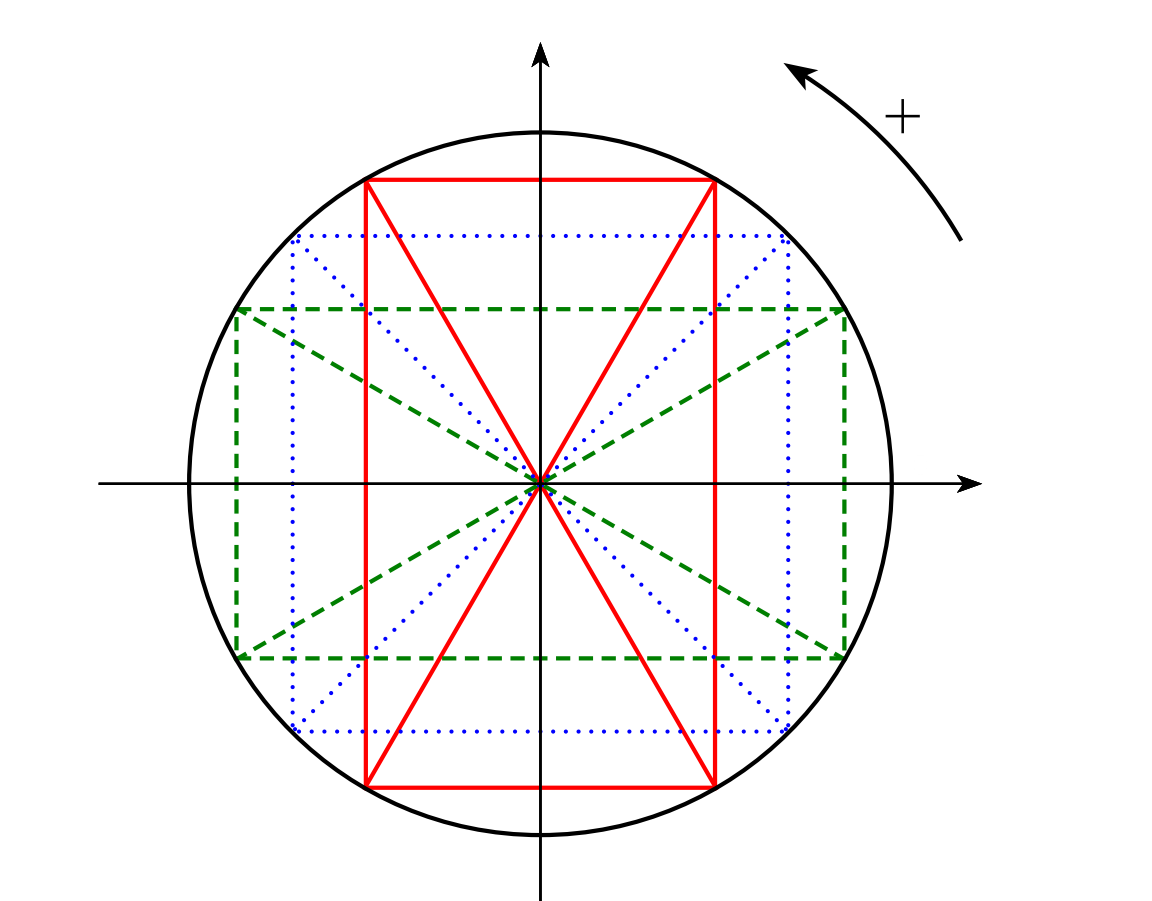
\includegraphics[scale=0.8]{../cercle_trigo}
	\end{figure}
	\end{center}
\end{exercice}
	
\end{document}